The first page you will notice when you visit the Geospatial Data Processor and Visualizer website will be the welcome screen. This is the screen each user will need to use to register and login. The page is shown in the picture below.\\[0.5cm]
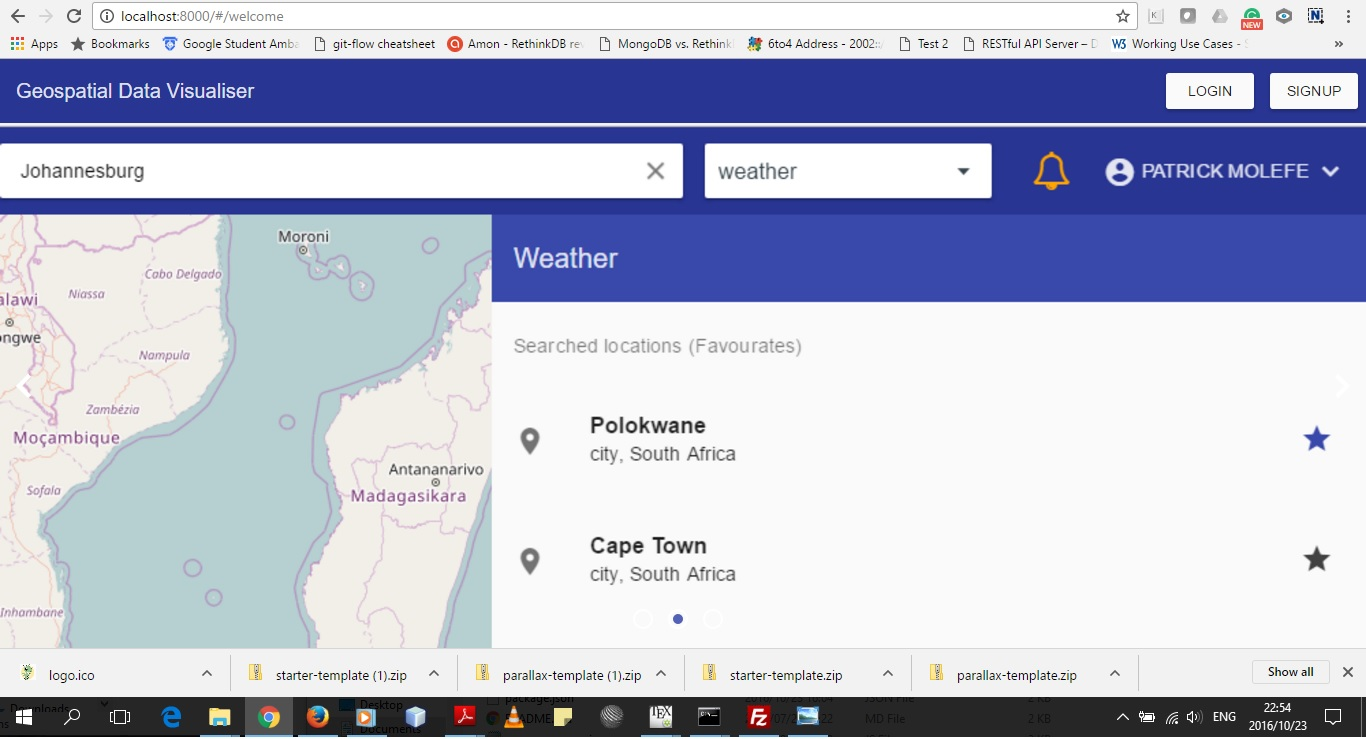
\includegraphics[width=\textwidth]{landingPage} \\[0.5cm]


Once you have logged onto the site you will land on the page shown below. The purpose of this section is to describe what each of the labelled functions are used for. \\[0.5cm]
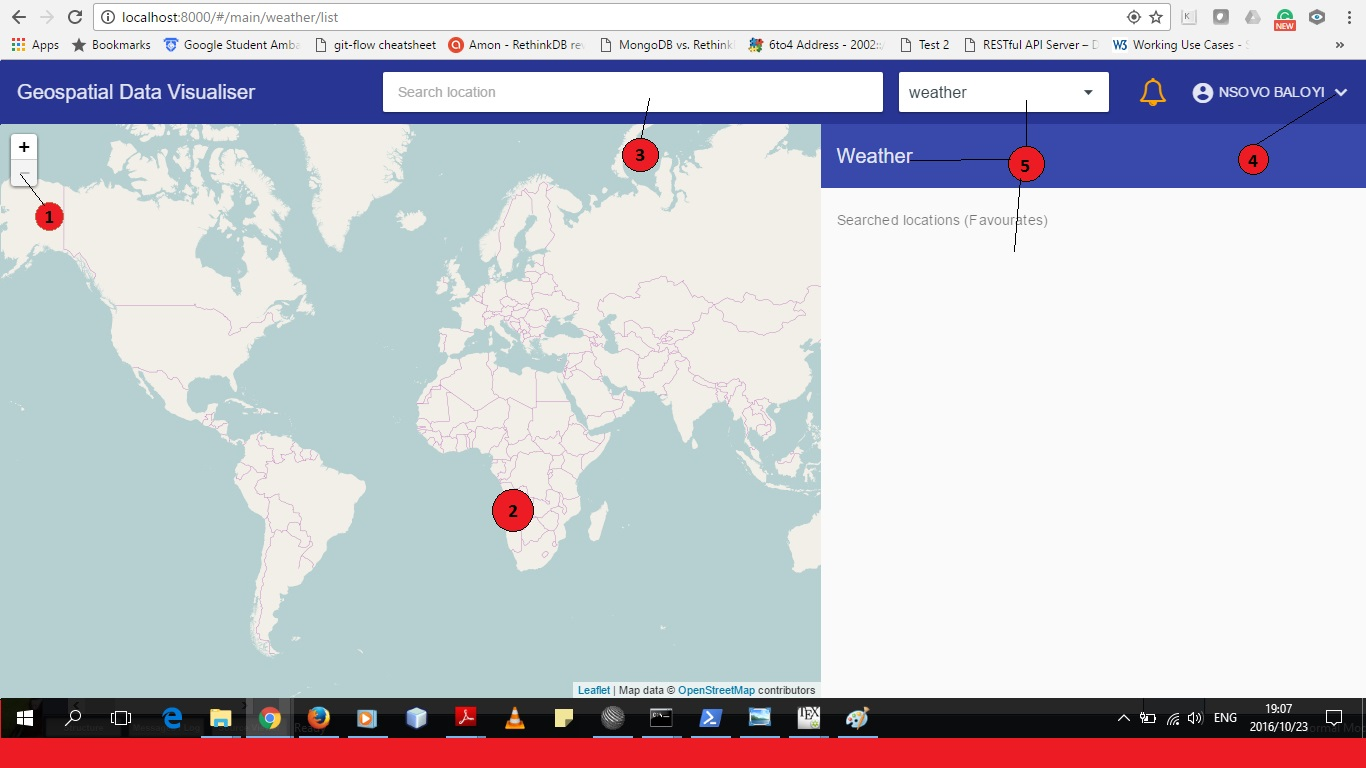
\includegraphics[width=\textwidth]{landingPage2} \\[0.5cm]

\begin{enumerate}
	\item \textbf{Zoom Button} : With the zoom button feature, one may zoom, the map area, in and out. The "-" button is used for the function of zooming the map area out, and the "+" button is used for the function of zooming the map area in.
	\item \textbf{Map Area} : Display the map
	\item \textbf{Search Area} : Used to search for any location in the world
	\item \textbf{User menu} : The user menu is used to log the user out as well as change an existing password.
	\item \textbf{Center Navigation} : The Dropdown area is used to choose which functionality, of the site, you'd like to use. When loaded, the site lands on the weather center by default.
\end{enumerate}
